% Chapter 25
\newprob{1718629061}
{
    % Active Physics p47 q1
    \def\tempf\ce{^{214}_{82}Pb}
    鉛-214 (\ce{^{214}_{82}Pb})進行$\beta$衰變而成為核素$X$。下列哪 一條方程正確顯示該衰變過程?
    \begin{tasks}
        \task \ce{^{214}_{82}Pb + $\beta$ -> ^{215}_{82}X}
        \task \ce{^{214}_{82}Pb + $\beta$ -> ^{214}_{83}X}
        \task \ce{^{214}_{82}Pb -> ^{214}_{83}X + $\beta$}
        \task \ce{^{214}_{82}Pb -> ^{215}_{83}X + $\beta$}
    \end{tasks}
}{C}

\newprob{1718631737}
{
% Active Physics p47 q2
以下的方程顯示某衰變系的其中一部分。
\ce{V ->[$\beta$] W ->[$\beta$] X ->[$\alpha$] Y ->[$\alpha$] Z}
哪些核素是同一元素的同位素?
\begin{tasks}
    \task V 和 Y
    \task W 和 Z
    \task V、W 和 X
    \task W、X 和 Z
\end{tasks}

}{A}

\newprob{1718632040}
{
    % Active Physics p47 q3
    一顆 \ce{^{237}_{93}Np} 原子核進行一系列衰變後變為一顆 \ce{^{209}_{83}Bi} 原子核。整個衰變過程總共會放出多少顆$\alpha$和$\beta$ 粒子?
    \begin{tasks}
        \task [] $\alpha$粒子數目\tab $\beta$粒子數目
        \task 6\tab 5
        \task 7\tab 4
        \task 7 \tab 5
        \task 8\tab 6
    \end{tasks}
}{B}

\newprob{1718632203}
{
    % Active Physics p47 q4
    釙(Po)的一種放射性同位素會進行一次$\alpha$衰變和 一次$\beta$衰變而成為核素$X$。下圖顯示釙的質量數 和原子序數。
    \par{\par\centering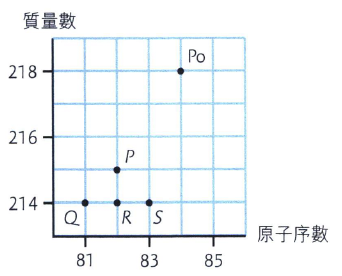
\includegraphics[width=.3\textwidth]{./img/ch1_prop_mc_2024-06-17-21-50-56.png}\par}
    圖中哪一點代表核素$X$?
    \begin{tasks}
        \task $P$
        \task $Q$
        \task $R$
        \task $S$
    \end{tasks}

}{D}

\newprob{1718632294}
{
    % Active Physics p47 q5
    下列哪些關於$\alpha$ 和 $\gamma$輻射的敍述正確?
    \begin{statements}
        \task 兩者皆能在真空中傳播。
        \task 兩者皆會被鉛板完全阻擋。
        \task 兩者皆會在電場中偏轉。
    \end{statements}
    \begin{tasks}
        \task 只有(1)
        \task 只有(3)
        \task 只有(1)和(2)
        \task 只有(2)和(3)
    \end{tasks}
}{A}

\newprob{1718632359}
{
    % Active Physics p47 q6
    某放射源只放出$\alpha$輻射,而不會放出$\beta$或$\gamma$輻 射。下列哪些有關放射源所放出輻射的敘述足以 證明這一點?
    \begin{statements}
        \task 輻射移向帶負電的金屬板。
        \task 輻射被5 mm 厚的鋁片完全阻擋。
        \task 輻射在擴散雲室中只產生既粗且直的徑跡。
    \end{statements}
    \begin{tasks}
        \task 只有(1)和(2)
        \task 只有(1)和(3)
        \task 只有(2)和(3)
        \task (1), (2) 和 (3)
    \end{tasks}
}{B}

\newprob{1718632437}
{
    % Active Physics p47 q7
    下圖顯示用絕緣細線將兩帶電的金 屬球$P$和$Q$懸掛,$P$帶正電荷而$Q$帶負電荷。 將一個$\alpha$ 放射源移近但不接觸金屬球,以下哪一 幅圖顯示一段時間之後的情況?
    \par{\par\centering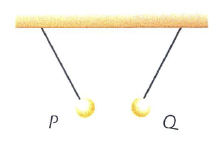
\includegraphics[width=.3\textwidth]{./img/ch1_prop_mc_2024-06-17-21-54-33.png}\par}
    \begin{tasks}(2)
        \task \topalign{\par\centering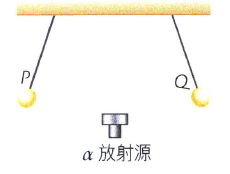
\includegraphics[width=.25\textwidth]{./img/ch1_prop_mc_2024-06-17-21-54-54.png}\par}
        \task \topalign{\par\centering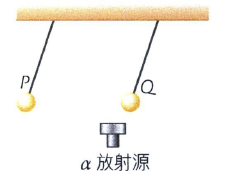
\includegraphics[width=.25\textwidth]{./img/ch1_prop_mc_2024-06-17-21-55-02.png}\par}
        \task \topalign{\par\centering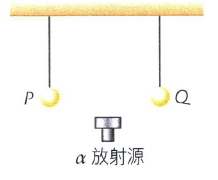
\includegraphics[width=.25\textwidth]{./img/ch1_prop_mc_2024-06-17-21-55-10.png}\par}
        \task \topalign{\par\centering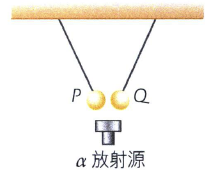
\includegraphics[width=.25\textwidth]{./img/ch1_prop_mc_2024-06-17-21-55-17.png}\par}
    \end{tasks}

}{
    C
}